\documentclass[12pt,a4paper]{scrartcl}
\usepackage{url, booktabs,pdflscape}
\usepackage[final]{pdfpages}
\usepackage[colorlinks]{hyperref}
\title{Student Robotics Competition Risk Assessment Form}

\begin{document}
\maketitle

\begin{description}
\item[Activity being assessed:] Student Robotics Competition 2013 (13/04/2013, 14/04/2013)
\item[Location:] Garden Court, Building 40, Highfield Campus, University of Southampton (\url{http://data.southampton.ac.uk/building/40.html})
\item[Who is exposed to the hazard:] Competitors, Teachers, Mentors
\end{description}

\begin{description}
\item[Assessor's name:]
\item[Assessor's job title:]
\item[Assessor's signature:]
\item[Date of assessment:]
\end{description}
\clearpage

\newcommand{\risk}[3]{
 #1 & #2 & #3 \\
}

\begin{landscape}
\section{Risks}
The following risks have been considered for the student robotics competition.  Further description of the meaning of risk ratings (presented in this section as $L \times S$) can be found in the next section.

A safety briefing will be given on all mornings, covering the points below.

\bigskip
\begin{tabular*}{\linewidth}[c]{p{14em}p{30em}c}
\toprule
\textbf{Hazard} & \textbf{Control Measures} & \textbf{Risk Rating} \\
\midrule

\risk{Electrical extension cable trip hazard}
{Cables taped down, kept near walls where practical.}
{2}

\risk{Injury while using power or manual tools}
{Teachers to supervise all use of tools given that teams bring their own. These tools are used at the teams own risk. Student Robotics will not provide tools at the competition.}
{3}

\risk{Electric shock by contact between water, electrical output and human}
{Water and electrical outputs kept strictly apart. Food and Drink is not allowed in the pit areas (i.e. places where teams work on their robots), or around the arena.}
{3}

\risk{Risk of Fire}
{No naked flames are allowed to be used intentionally. If a fire breaks out accidentally, University of Southampton Regulations will be followed as detailed below.}
{2}

\risk{Risk of falling objects from arena}
{The arena is designed to tolerate reasonable additional weight. It is built out of building scaffolding. All objects are securely attached but may become loose if tampered with. Competitors will not be permitted in the arena without supervision, and Student Robotics will endeavour to remove any person using the arena as a climbing frame or tampering with the equipment attached to it.}
{4}

\risk{Interaction with robots: electric shock, minor injury}
{Competitors are only allowed into the arena with a mentor present, but may only work on robots in their pits. Robots may only be tested under supervision and if robot safety rules are met (see rulebook 2.10-2.14, 2.16, 2.17). Electronics provided by Student Robotics are housed in a plastic casing, and wiring will be inspected by a member of Student Robotics before competitors are allowed to work on their robots.  Rulebook: \url{https://www.studentrobotics.org/resources/2012/rulebook.pdf}}
{1}

\risk{Misuse of batteries}
{For the duration of the competition, Student Robotics will handle charging of the batteries and will be collecting spare batteries and chargers from teams on entry. Student Robotics will be charging batteries in a safe zone away from the main competition area and inaccessible to competitors, and the batteries will be charged by trained Student Robotics personnel in the manner described in \url{https://www.studentrobotics.org/docs/kit/batteries}}
{3}
\bottomrule
\end{tabular*}
\end{landscape}

\begin{landscape}

\section{Assessment Guidance}

The risk ratings of the risks in the previous section are calculated by multiplying $L$, the likelihood rating, by $S$, the severity rating.

\bigskip
\begin{minipage}[b]{0.5\linewidth}
\begin{tabular}[c]{lc}
\hline
  \textbf{Likelihood} & \textbf{Likelihood rating} \\
\hline
  Very unlikely & 1 \\
  Unlikely & 2 \\
  Likely & 3 \\
  Fairly likely & 4 \\
  Very likely & 5 \\
\hline
\end{tabular}
\end{minipage}
\begin{minipage}[b]{0.5\linewidth}
\begin{tabular}[c]{lc}
\hline
  \textbf{Severity} & \textbf{Severity rating} \\
\hline
  First Aid injury/illness & 1 \\
  Minor injury/illness & 2 \\
  `3 day' injury/illness & 3 \\
  Major injury/illness & 4 \\
  Fatality/disabling injury & 5 \\
\hline
\end{tabular}
\end{minipage}
\bigskip

The following should be used to rate the risk and plan corrective action:
\bigskip
\newcommand{\riskinfo}[4]{
  #1 & #2 & #3 & #4 \\
}

\begin{tabular*}{\linewidth}[c]{cccp{33em}}
\hline
  \textbf{Risk Rating} & \textbf{Category} & \textbf{Tolerability} & \textbf{Comments} \\
\hline

  \riskinfo{1--2}{Very Low}{Acceptable}
  {No further action is necessary other than to ensure that the controls are maintained.}

  \riskinfo{3--4}{Low}{Acceptable}
  {No additional controls are required unless they can be implemented at very low cost (in terms of time, money and effort).}

  \riskinfo{5--7}{Medium}{Tolerable}
  {Consideration should be given as to whether the risks can be lowered, where applicable, to a tolerable level, and preferably acceptable level, but the costs of additional risk reduction measures should be taken into account.  The risk reduction measures should be implemented within a defined time period.}

  \riskinfo{8--14}{High}{Tolerable}
  {Substantial efforts should be made to reduce the risk.  Risk reduction measures should be implemented urgently within a defined time period and it might be necessary to consider suspending or restricting the activity, or to apply interim risk control measures, until this has been completed. Considerable resources might have to be allocated to additional control measures.}

  \riskinfo{15 and above}{Very High}{Unacceptable}
  {Substantial improvements in risk control are necessary, so that risk is reduced to a tolerable or acceptable level.}

\hline
\end{tabular*}

\end{landscape}


\clearpage

\newpage
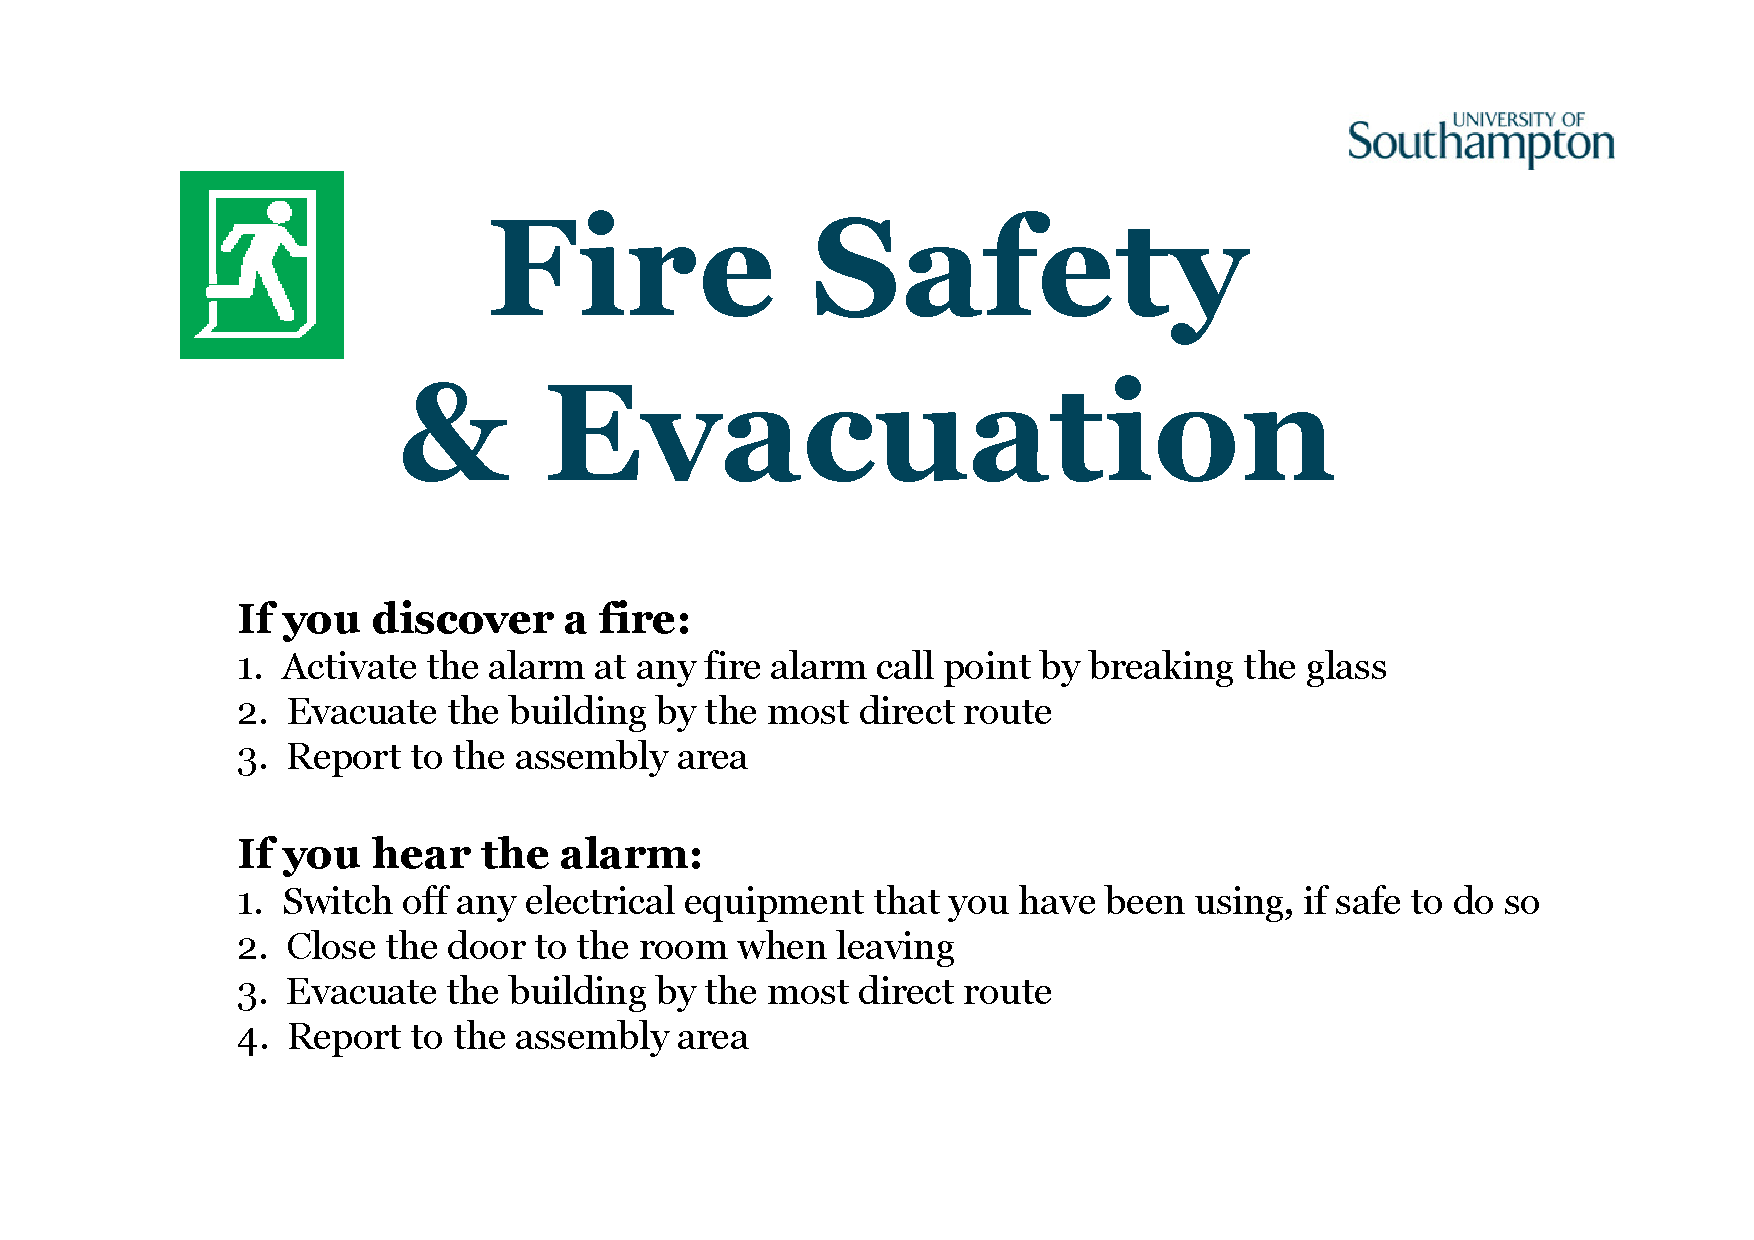
\includepdf[scale=1.0,landscape]{Fire1.pdf}
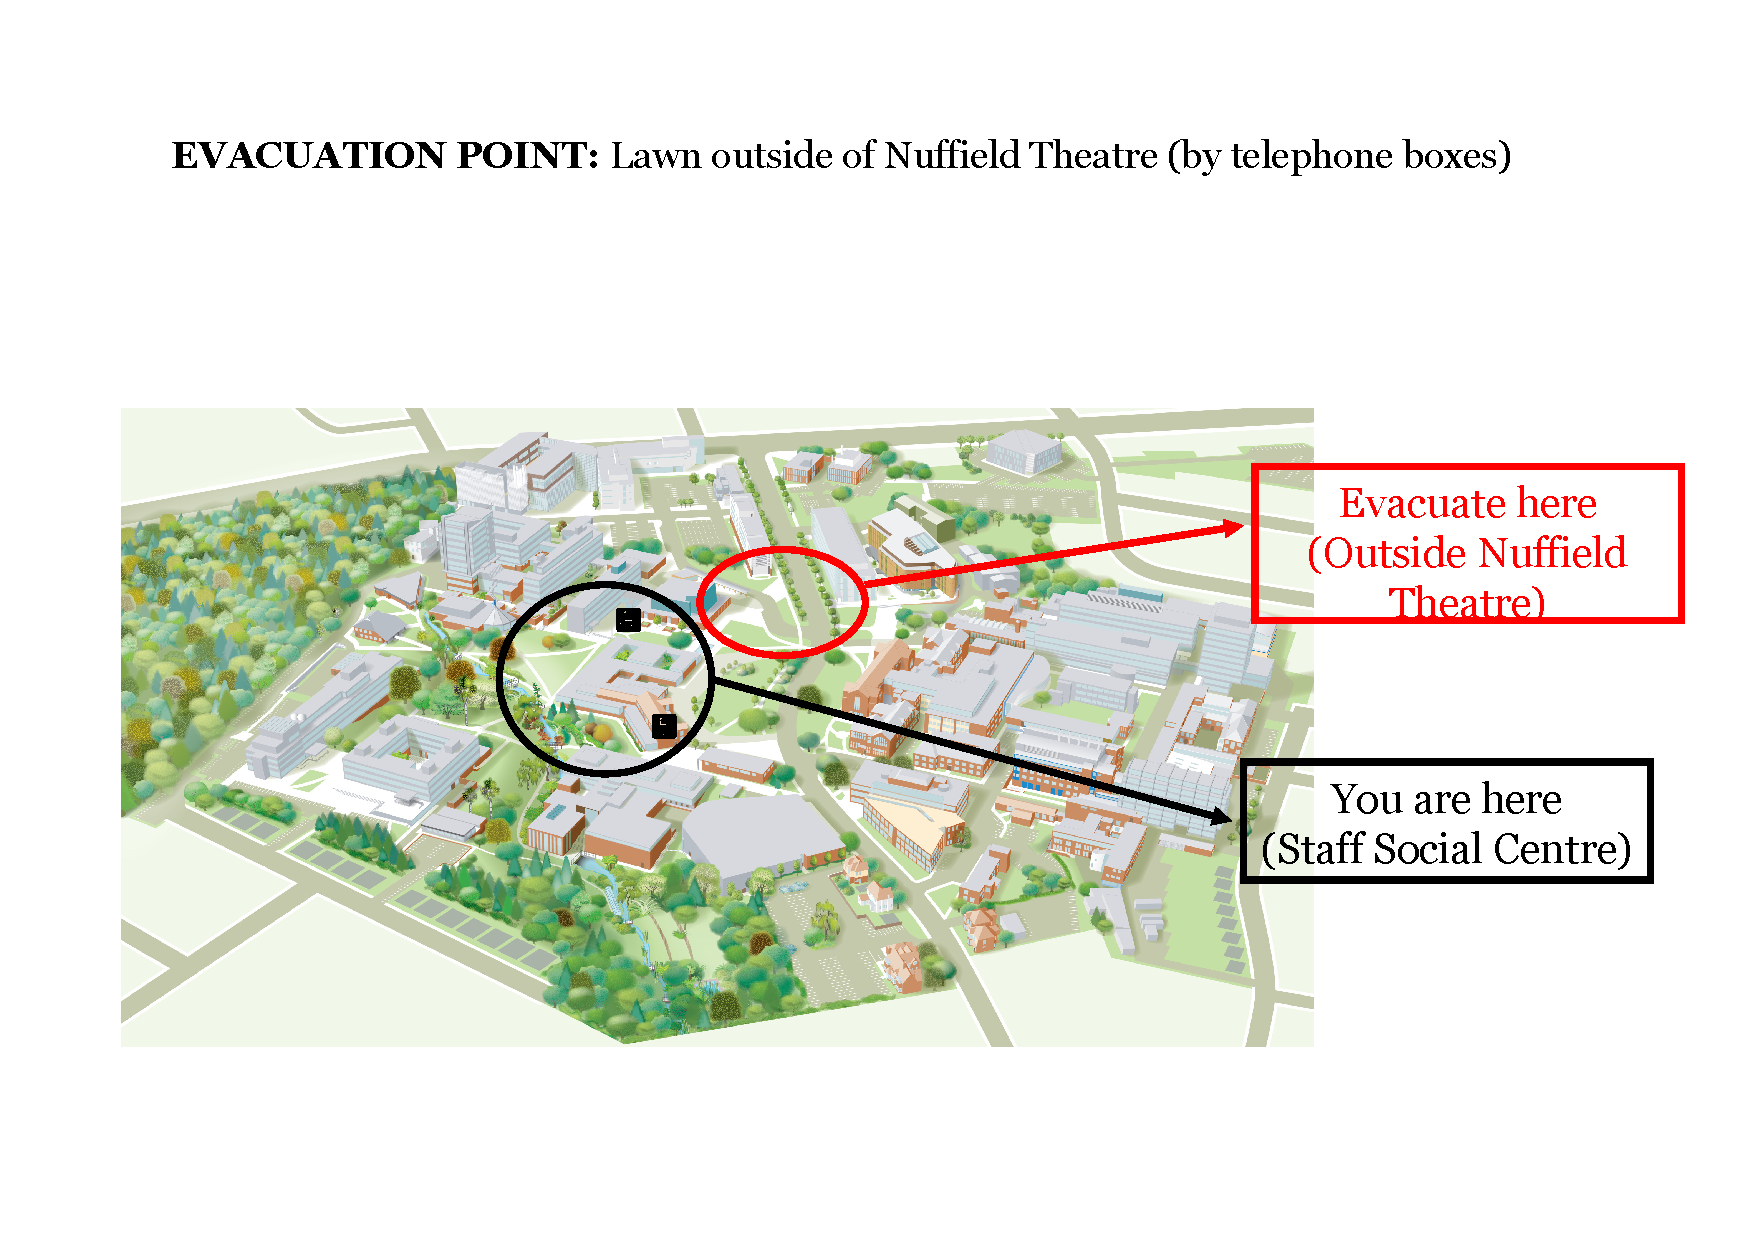
\includepdf[scale=1.0,landscape]{Fire3.pdf}

\end{document}

